\documentclass[a4paper,12pt]{article}
%%%%%%%%%%%%%%%%%%%%%%%%%%%%%%%%%%%%%%%%%%%%%%%%%%%%%%%%%%%%%%%%%%%%%%%%%%%%%%%%%%%%%%%%%%%%%%%%%%%%%%%%%%%%%%%%%%%%%%%%%%%%%%%%%%%%%%%%%%%%%%%%%%%%%%%%%%%%%%%%%%%%%%%%%%%%%%%%%%%%%%%%%%%%%%%%%%%%%%%%%%%%%%%%%%%%%%%%%%%%%%%%%%%%%%%%%%%%%%%%%%%%%%%%%%%%
\usepackage{eurosym}
\usepackage{vmargin}
\usepackage{amsmath}
\usepackage{graphics}
\usepackage{epsfig}
\usepackage{enumerate}
\usepackage{multicol}
\usepackage{subfigure}
\usepackage{fancyhdr}
\usepackage{listings}
\usepackage{framed}
\usepackage{graphicx}
\usepackage{amsmath}
\usepackage{chngpage}
%\usepackage{bigints}

%%\usepackage{fontspec}


\usepackage{vmargin}
% left top textwidth textheight headheight
% headsep footheight footskip
\setmargins{2.0cm}{2.5cm}{16 cm}{22cm}{0.5cm}{0cm}{1cm}{1cm}
\renewcommand{\baselinestretch}{1.3}

\setcounter{MaxMatrixCols}{10}
\begin{document}
	%%--- Higher Certificate, Paper II, 2003. Question 4
	%%%%%%%%%%%%%%%%%%%%%%%%%%%%%%%%%%%%%%%%%%%%%%%%%%%%%%%%%%%%%%%%%%%%%%%%%%%%%%%%%%%%%%%%%%%%%%%%%%%%%%%%%%%%%%%%%%%%%%%%%%%%%%%%%
	
	\large 
	\noindent A psychologist claims that visual memory is more effective than aural memory.  To test this claim, ten students are selected at random and examined for visual and aural memory using a standard memory test.  For each student, the psychologist notes whether his or her aural (A) or visual (V) memory score is the greater.  The results are as follows. 
	\begin{center}
		\begin{tabular}{|c||c|c|c|c|c|c|c|c|c|c|} 
			\hline 
			Student & 1 & 2 & 3 & 4 & 5 & 6 & 7 & 8 & 9 & 10\\ \hline 
			Test & A&  V&  V&  A & V & V & V & A & V & V \\ \hline 
		\end{tabular}
	\end{center}
	
	\begin{table}[ht!]
		
		\centering
		
		\begin{tabular}{|p{15cm}|}
			
			\hline  
			
			\large  
			Carry out a suitable analysis of these data to investigate the psychologist’s claim and comment on your results. 
			
			
			\\ \hline
			
		\end{tabular}
		
	\end{table}
	\bigskip 
	
	\large
	\noindent A sign test is appropriate, the null hypothesis being that A and V are equally
	likely. Hence the number of As is binomial with parameters
	10 and 1/2, as is the number of Vs, if the null hypothesis is true. The alternative
	hypothesis claims that V is greater. A one-sided test is therefore needed.
	The observed results are $n_A = 3$, $n_B = 7$.
	\begin{framed}
		\[P( n_i \leq k) =  \left[ \sum^{k}_{i=0}  { n \choose i} \right] \times \frac{1}{2^n}\]
		\[P( n_i \geq k) =  \left[ \sum^{n}_{i=k}  { n \choose i} \right] \times \frac{1}{2^n}\]
	\end{framed}
	
	If the null hypothesis is true, we have
	
	
	
	\begin{eqnarray*}
		P( n_i \geq 7) &=& \left[ {10 \choose 7} +  {10 \choose 8} +  {10 \choose 9} +  {10 \choose 10} \right] \frac{1}{2^{10}}\\
		&=& \left[ 120 \;+\; 45 \;+\; 10 \;+\; 1 \right] \frac{1}{2^{10}}\\
		&=& 0.172\\
	\end{eqnarray*}
	%%%%%%%%%%%%%%%%%%%%%%%%%%%%%%%%%%%%%
	\begin{itemize}
		\item 
		There is not enough evidence to reject the null hypothesis.
		
	\end{itemize}
	
	
	\newpage
	\subsection*{Part (b)}
	\large
	\noindent After completing this experiment, the psychologist decides to investigate whether aural memory scores can be improved by coaching.  A second experiment is conducted in which a random sample of 12 students perform an aural memory test before and after several sessions of coaching in skills believed to aid aural memory.  The results of the two tests are as follows. \\ \medskip
	\begin{center}
		\begin{tabular}{|c||c|c|c|c|c|c|c|c|c|c|c|c|} \hline
			Student &(1)& (2) &(3) &(4) &(5) &(6) &(7) &(8)& (9)& (10)& (11)& (12)\\  \hline
			Before & 53 & 59 & 61 & 48 & 39 & 56 & 75 & 45 & 73 & 60 & 69 & 66 \\ \hline 
			After & 60 & 57 & 67 & 52 & 63 & 71 & 70 & 46 & 76 & 65 & 62& 65\\ \hline 
		\end{tabular}
	\end{center}
	\begin{table}[ht!]
		
		\centering
		
		\begin{tabular}{|p{15cm}|}
			
			\hline   \large
			\begin{enumerate}[(i)]
				\item  It is required to test whether aural memory is improved, using a nonparametric test.  Explain why it is not satisfactory to use a test similar to the one used in part (a).  Carry out an appropriate non-parametric test. 
				\item It is suggested that a parametric test would be more appropriate to analyse the data.  Without performing the analysis, state which test you would use and any assumptions necessary for this analysis to be valid.  Would these assumptions be reasonable in this case? 
			\end{enumerate}
			
			
			\\ \hline
			
		\end{tabular}
		
	\end{table}
	%%%%%%%%%%%%%%%%%%%%%%%%%%%%%%%%%%%%%%%%%%%%%%%%%%%%%%%%%%%%%%%%%%%%%%%%%%%%%%%%%%
	\newpage
	\begin{itemize}
		\item The sign test is not very powerful. The sample size here (10) is not really large enough for its effective use.
		\item The data provide information which the sign test would not use,
		namely that measuring the change on a numerical scale.
		\item As well as the sign of the change we should use the magnitude. A Wilcoxon signed-rank
		test is suitable. 
		\item Difference $A \;-\; B$ are as follows, and the absolute
		values of the differences are ranked in size order, with tied values
		given their average ranking.
	\end{itemize}
	%%%%%%%%%%%%%%%%%%%%%%%%%%%%%%%%%%%%%%%%%%%%%%%%%%%%%%%%%%%%%%%%%%%%%%%%%%%%%%%%%%%%%%%%%%%%%%%%%%%%%%%%%%%%%%%%%%%%%%%%%%%%%%%%%
	
	
	\begin{center}
		\begin{tabular}{|c|c|c|c|c|c|c|c|c|c|c|c|c|} \hline 
			Student &(1)& (2) &(3) &(4) &(5) &(6) &(7) &(8)& (9)& (10)& (11)& (12)\\ \hline 
			Difference & 7 & - 2 & 6 & 4 & 24 & 15 & - 5 & 1 & 3 & 5 & - 7& - 1 \\  \hline 
			$|\mbox{Diff}|$ & 7 &  2 & 6 & 4 & 24 & 15 &  5 & 1 & 3 & 5 & 7&  1 \\  \hline 
			Rank &${ \displaystyle  9 \frac{1}{2} }$  & 3 & 8 & 5 & 12 & 11 &${ \displaystyle  6\frac{1}{2} }$  & ${ \displaystyle 1\frac{1}{2} }$  & 4 & ${ \displaystyle 6\frac{1}{2}}$  & ${ \displaystyle 9\frac{1}{2} }$  & ${ \displaystyle 1\frac{1}{2} }$  \\ \hline 
		\end{tabular}
	\end{center}
	\newpage
	\bigskip 
	\begin{itemize}
		\item 
		The null hypothesis is that aural memory scores are not altered by
		coaching, the alternative hypothesis is that coaching leads to
		improvement. A one-sided test is required.
		\item 
		The sum of ranks of negative values is $T-  = 20\frac{1}{2}$ and of positive values
		is $T+ = 57\frac{1}{2} $. 
		\item We use $T = \mbox{min}(T- , T+) = 20\frac{1}{2}$. 
		\item Tables for $n = 12$ give 17
		as the critical value for a one-sided 5\% test, so there is not enough
		evidence to reject the null hypothesis.
		\item A paired-samples $t-$test using the differences would be appropriate if
		the distribution of differences appeared to be approximately Normal.
		\item The two large values for (5) and (6) make this unlikely, both being on
		the same side (+). It would be unwise to use the $t-$test in this case.
	\end{itemize}
	
	\newpage
	
	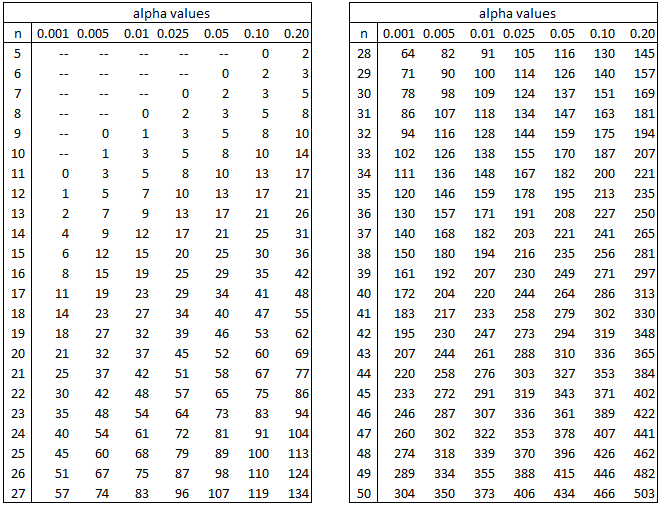
\includegraphics[]{images/signed-ranks-table.png}
	\newpage
	
	\begin{table}[ht!]
		
		\centering
		
		\begin{tabular}{|p{15cm}|}
			
			\hline  
			
			\\ \hline
			
		\end{tabular}
		
	\end{table}
	
\end{document}
